% ------------------------------------------------------------------------------
% TYPO3 v9 LTS - What's New (English Version)
%
% @author	Michael Schams <schams.net>
% @license	Creative Commons BY-NC-SA 3.0
% @link		https://typo3.org/help/documentation/whats-new/
% @language	English
% ------------------------------------------------------------------------------

\section{Backend User Interface}
\begin{frame}[fragile]
	\frametitle{Backend User Interface}

	\begin{center}\huge{\color{typo3darkgrey}\textbf{Backend User Interface}}\end{center}
	\begin{center}\large{\textit{The TYPO3 administration interface is now better than ever}}\end{center}

\end{frame}

% ------------------------------------------------------------------------------
% Page Tree

\begin{frame}[fragile]
	\frametitle{Backend User Interface}
	\framesubtitle{Page Tree}

	\begin{itemize}
		\item Page tree is now based on SVGs and features superfast rendering times
		\item All ExtJS code has been removed completely from the TYPO3 backend
		\item Delete page by simply moving them to the right
	\end{itemize}

	\begin{figure}
		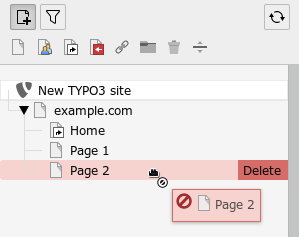
\includegraphics[width=0.3\linewidth]{BackendUserInterface/DeletePageInPageTree.png}
	\end{figure}

\end{frame}

% ------------------------------------------------------------------------------
% Page Tree

\begin{frame}[fragile]
	\frametitle{Backend User Interface}
	\framesubtitle{Modal Windows}

	\begin{itemize}
		\item TYPO3 now uses modal windows consistently in the backend
		\item This ensures a smooth and non-interruptive interaction with the system
		\item For example, when adding a new content element:
	\end{itemize}

	\begin{figure}
		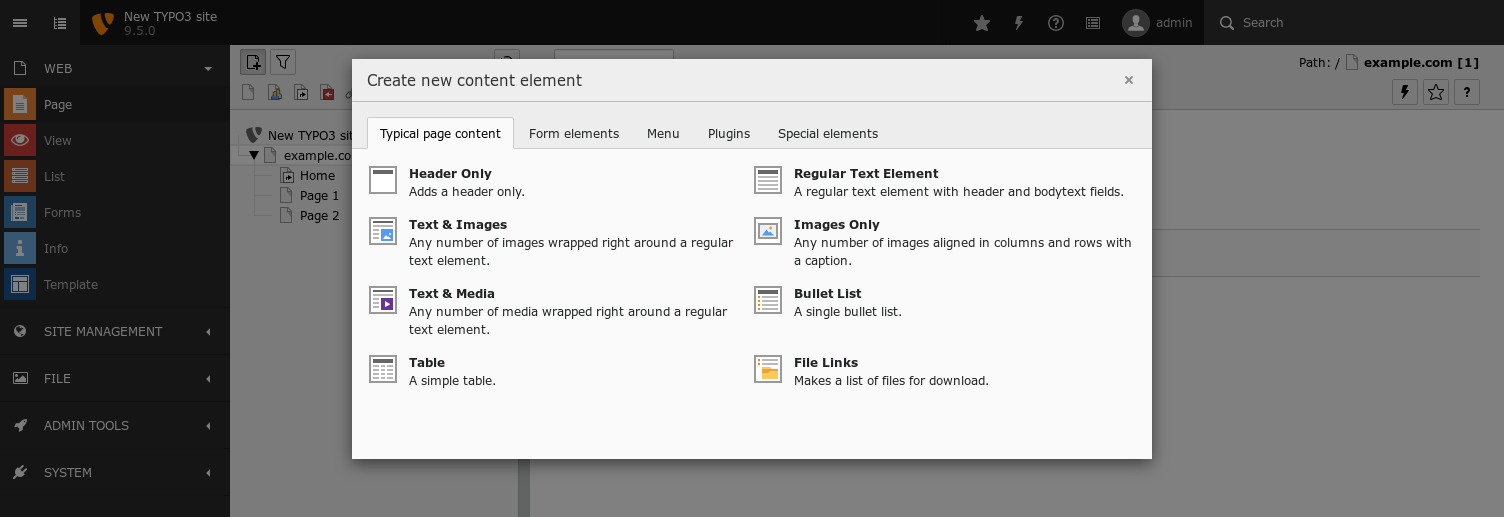
\includegraphics[width=0.85\linewidth]{BackendUserInterface/ModalWindowNewContentElement.png}
	\end{figure}

\end{frame}

% ------------------------------------------------------------------------------
% Duplicate Content Elements
% #84749 - Hide "duplicate" button by default

\begin{frame}[fragile]
	\frametitle{Backend User Interface}
	\framesubtitle{Duplicate Content Elements}

	% decrease font size for code listing
	\lstset{basicstyle=\smaller\ttfamily}

	\begin{itemize}
		\item Button to duplicate a content element with a single mouse click
		\item Visibility can be configured in userTSConfig ("1" = enabled):

\begin{lstlisting}
options.showDuplicate = 1
options.showDuplicate.[table] = 1
\end{lstlisting}

	\end{itemize}
	\vspace{-0.5cm}
	\begin{figure}
		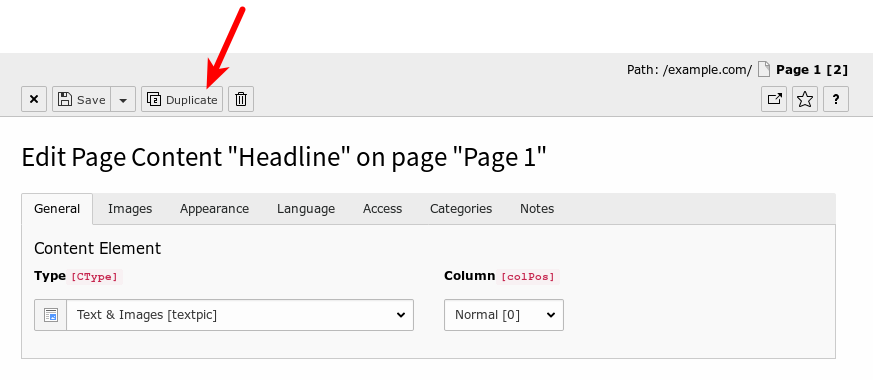
\includegraphics[width=0.8\linewidth]{BackendUserInterface/DuplicateButtonHiddenByDefault.png}
	\end{figure}

\end{frame}

% ------------------------------------------------------------------------------
% Further Improvements

\begin{frame}[fragile]
	\frametitle{Backend User Interface}
	\framesubtitle{Further Improvements}

	\begin{itemize}
		\item Images are now rotated automatically on upload/edit, based on
			their orientation stored in the EXIF metadata of the image
		\item "Toggle switches" have been introduced, which are also a useful
			tool to allow users to switch between two states easily
		\item Thumbnail images are now loaded asynchronously\newline
			\small(for example in the filelist)\normalsize
		\item In debug mode, the field name of every FormEngine field is shown
			to admin users in the backend\newline
			\small(see "In-Depth Changes" for an example)\normalsize
		\item and many more...
	\end{itemize}

\end{frame}

% ------------------------------------------------------------------------------
